% Created 2020-05-13 Wed 14:19
% Intended LaTeX compiler: pdflatex
\documentclass[unrestricted]{meetingnotesminutes}
                    \title{ {{{title}}} }
\author{ {{{author}}} }
\project{ {{{keyword(PROJECT)}}} }
\wheremeeting{ {{{keyword(LOCATION)}}} }
\whenmeeting{ {{{keyword(TIME)}}} }
\initiator{Vi Kumar}
\participant[present]{Abdullah Sherif - as394@hw.ac.uk}
\participant[present]{Vishakh Kumar - vpk2@hw.ac.uk}
\participant[present]{Vishnu Sarathy - vks2@hw.ac.uk}
\participant[information]{Dr Mehdi Nazarinia}
\participant[information]{Dr Ityonna Amber}
\author{Vi Kumar}
\date{\today}
\title{Mathworks Minidrone Competition}
\hypersetup{
 pdfauthor={Vi Kumar},
 pdftitle={Mathworks Minidrone Competition},
 pdfkeywords={},
 pdfsubject={},
 pdfcreator={Emacs 26.3 (Org mode 9.3.6)},
 pdflang={English}}
\begin{document}

\frontmatter

\section{Agenda}
\label{sec:org1afe350}

\section*{Agenda}
\begin{itemize}
  \item Housingkeeping \& Onboarding
  \item Explain basic model of drone control
  \item Assign tasks
\end{itemize}

\tasklist

\section{Housekeeping \& Onboarding}
\label{sec:orgc2b2f5b}

\subsection{Git Repository}
\label{sec:org88e5c06}
Get used to git because that's the easiest way for us to work together.
Great documentation at \url{https://git-scm.com/doc}

Quick reference:
git pull origin master
git add .
git commit -m "Useful message"
git push origin master

Our repo: \url{https://gitlab.com/grokkingStuff/MathWorksMiniDrone}

\task{Install git & create a gitlab account}{ Abdullah and Vishnu}{Soon}

\subsection{Onramp \& Competition Rules}
\label{sec:org720bfa5}
Would recommend reading the rules pdf
Finish off the Onramp and put your certificates to the git repo

\task{Post Onramp certificates to Gitlab Repo}{ Abdullah and Vishnu}{Soon}

\subsection{Useful Resources}
\label{sec:org4ee09d0}

Look these up and

\subsubsection{Youtube}
\label{sec:org3ebd9af}

Mostly Steve Brunton

\begin{enumerate}
\item Singular Value Decomposition
\label{sec:orgf14eb09}
\url{https://www.youtube.com/playlist?list=PLMrJAkhIeNNSVjnsviglFoY2nXildDCcv}

Useful for finding the "most important" eigenvalues. Used to find the most controllable regions of the drone

\item Control Bootcamp
\label{sec:orgc6cf82b}
\url{https://www.youtube.com/playlist?list=PLMrJAkhIeNNR20Mz-VpzgfQs5zrYi085m}

Useful for picking up basics of Control Theory
\end{enumerate}

\subsubsection{Research Papers}
\label{sec:orgcbd2972}

So I have zero real knowledge about Control Schemes. And that probably reflects in the literature review I've been doing - it's definitely possible and very likely that I'm missing on a bunch of research because I'm not familiar with field terminology

That said, hope these keywords help you out
\begin{itemize}
\item Visual-based
\item Line following
\item Line Following Robot (LFR)
\end{itemize}

Some papers I found useful were:

\begin{enumerate}
\item Eriksen 2014
\label{sec:org090d9e4}

Eriksen, Christopher \& Ming, Kristina \& Dodds, Zachary. (2014). Accessible Aerial Robotics. Journal of Computing Sciences in Colleges. 29. 218-227.

This work demonstrates some of the computational capabilities of the inexpensive AR.Drone2 quadcopter. Fundamentally a platform that navigates in 3D, the drone offers a clean interface to 2D sensor data through its video stream. By using image-matching to bridge that "interdimensional" gap, this work demonstrates that the drone offers an accessible, compelling platform for research and independent projects at any institution. In the process, we demonstrate that accessible physical platforms, i.e., the drone, the Kinect, and their scaffolding software, ROS, now offer capabilities with much wider curricular and computational applications.

\begin{verbatim}
@article{article,
author = {Eriksen, Christopher and Ming, Kristina and Dodds, Zachary},
year = {2014},
month = {04},
pages = {218-227},
title = {Accessible Aerial Robotics},
volume = {29},
journal = {Journal of Computing Sciences in Colleges}
}
\end{verbatim}


\item Mur-Artal 2015
\label{sec:orgaf6aefe}

ORB-SLAM2 is a real-time SLAM library for Monocular, Stereo and RGB-D cameras that computes the camera trajectory and a sparse 3D reconstruction (in the stereo and RGB-D case with true scale). It is able to detect loops and relocalize the camera in real time. We provide examples to run the SLAM system in the KITTI dataset as stereo or monocular, in the TUM dataset as RGB-D or monocular, and in the EuRoC dataset as stereo or monocular. We also provide a ROS node to process live monocular, stereo or RGB-D streams. The library can be compiled without ROS. ORB-SLAM2 provides a GUI to change between a SLAM Mode and Localization Mode, see section 9 of this document.

\begin{verbatim}
@article{murTRO2015,
  title={{ORB-SLAM}: a Versatile and Accurate Monocular {SLAM} System},
  author={Mur-Artal, Ra\'ul, Montiel, J. M. M. and Tard\'os, Juan D.},
  journal={IEEE Transactions on Robotics},
  volume={31},
  number={5},
  pages={1147--1163},
  doi = {10.1109/TRO.2015.2463671},
  year={2015}
 }
\end{verbatim}
\end{enumerate}

\section{Action items}
\label{sec:orgf1856e3}
\subsection{Need to get real-life data for stuff}
\label{sec:org5097b67}
Need to get Dr Mehdi to send over a recording of sensor data from the drone. While we can't actually work with said drone thanks to the whole lockdown, having some raw data should allow us to make (somewhat rational) decisions about which filters and what parameters to use to analyze said data.

Not a priority (yet) and I think Dr Mehdi is busy with exam stuff. Would recommend bugging him about it before our meeting on May 17.

\subsection{Need to copy equations of motion from hastily written notes to an actual file}
\label{sec:org4bf350f}

For the UKF because you need a proper statespace model
\subsubsection{Need to also add a real simple Simulink implementation of the statespace model you're using. Need some controlability analysis}
\label{sec:orgc0e0414}

Mostly so that we know we're not missing out on some really useful info

\section{Current Status of Project}
\label{sec:org4444499}
\subsection{Mission Timeline}
\label{sec:orga232f7c}

\begin{itemize}
\item Take off from a circular pad
\item Follow a track laid on floor
\begin{itemize}
\item Track sections have straight lines with no curves
\item Downward facing camera to track lines
\end{itemize}
\item Land on circular end marker
\end{itemize}

GPS-denied environment and all calculations must be done on-board

Time considered only when the minidrone lands on the end marker.
In order for the minidrone to be considered as having landed:
\begin{itemize}
\item Minidrone must be upright.
\item Minidrone's bottom surface has to touch the floor.
\end{itemize}
\begin{center}
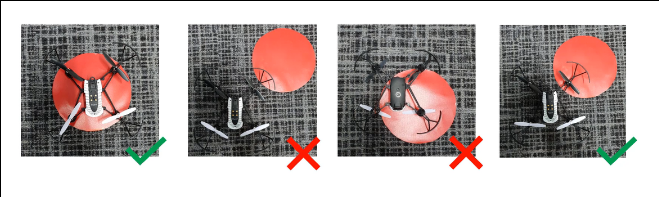
\includegraphics[width=.9\linewidth]{./images/screenshot-01.png}
\end{center}

\subsection{General Software Stack}
\label{sec:org8c4f416}

Work off ROS inside Simulink.

\begin{itemize}
\item Why?
\end{itemize}
Plenty of existing models in ROS that are industry-tested. Also, it's usually been optimized for the purpose and the ability to just subscribe to a node that gives you information is crazy useful

\begin{itemize}
\item So why Simulink?
\end{itemize}
The control logic is best expressed in Simulink because writing C code that has a decent state machine AND is able to interface with ROS nodes AND is able to help us out with a GUI/debug tools IS HARD! Simulink acts as a glue between our hardware, voodoo blackbox, and our ideas.


\subsubsection{Matlab/Simulink}
\label{sec:org5e90514}
Not gonna write much here because I think everyone is familiar with it
\subsubsection{ROS}
\label{sec:org9490141}
Robot Operating System (ROS) is a framework of tools, libraries, and software to aid in robot software development. It is a flexible system for programming robots and controlling robotic platforms. ROS was developed by an open-source collaborative community to help grow the world of robotics. Applications for working with hardware, robotic simulation models, path planning, localization and mapping, and many other algorithms are available. For an introduction to ROS, see the ROS Introduction on their website.

\begin{enumerate}
\item ROS Toolbox in Simulink
\label{sec:org3bcf87f}

\url{https://www.mathworks.com/help/ros/gs/robot-operating-system-ros.html}

ROS Toolbox allows you to access ROS functionality in MATLAB®. Use MATLAB to communicate with a ROS network, interactively explore robot capabilities, and visualize sensor data. You can develop robotics applications by exchanging data with ROS-enabled robots and robot simulators such as Gazebo. You can also create Simulink® models that exchange messages with a ROS network. Verify your model within the Simulink environment by receiving messages from, and sending messages to, ROS-enabled robots and robot simulators. From your model, you can also generate C++ code for a standalone ROS application.

Both MATLAB and Simulink support the TCPROS transport layer (see TCPROS). The UDPROS transport is not supported.

ROS Toolbox supports ROS Indigo and Hydro platforms, but your own ROS installation may have different message versions. If you would like to overwrite our current message catalog, you can utilize ROS Custom Message Support to generate new message definitions. For ROS 2, ROS Toolbox supports the Dashing Diademata platform.
\end{enumerate}

\subsection{Drone Finite State Machine}
\label{sec:org98f7613}


\begin{center}
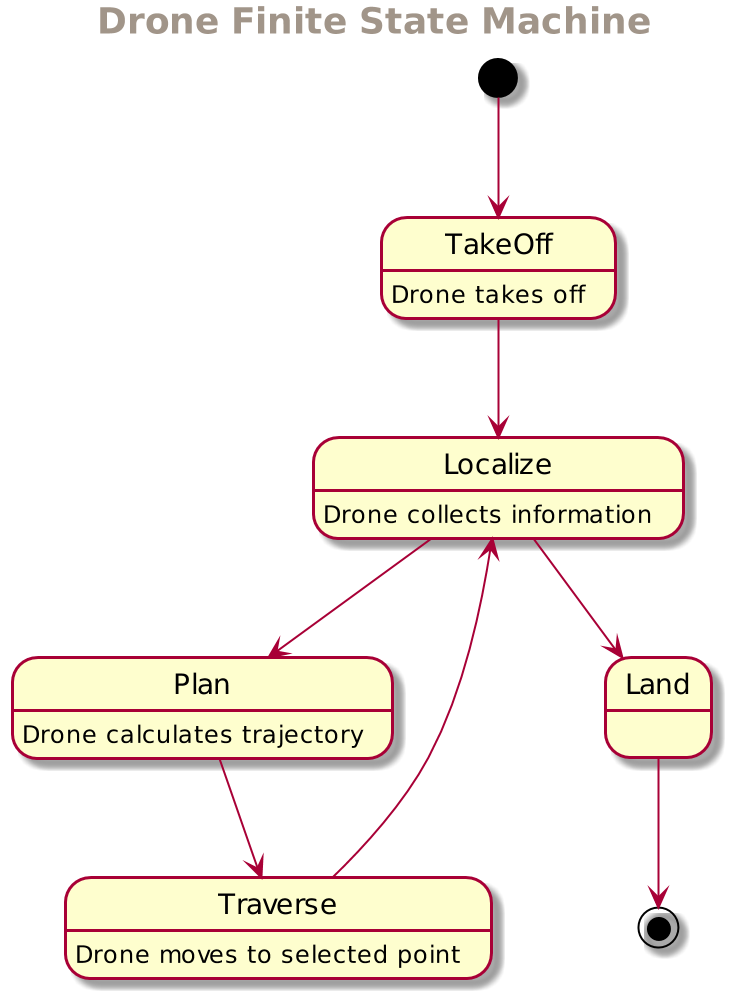
\includegraphics[width=.9\linewidth]{drone-fsm.png}
\end{center}

So our drone needs a way to figure out what to do and how to do it.
A really simple Finite State Machine is below. Should probably ask someone who knows what they're doing.

The SLAM algorithm is commputer intensive BUT once localization is done, it's pretty fast.

So our first pass will be super slow to collect info.
Then, we can use the state machine to switch between the Localize \& Traverse states and make optimal use of information.

\subsection{ORB-SLAM2}
\label{sec:orgdfffd46}


Github-Repo: \url{https://github.com/raulmur/ORB\_SLAM2}
Youtube-Example: \url{https://www.youtube.com/watch?v=IuBGKxgaxS0}

\begin{quote}
ORB-SLAM2 is a real-time SLAM library for Monocular, Stereo and RGB-D cameras that computes the camera trajectory and a sparse 3D reconstruction (in the stereo and RGB-D case with true scale). It is able to detect loops and relocalize the camera in real time. We provide examples to run the SLAM system in the KITTI dataset as stereo or monocular, in the TUM dataset as RGB-D or monocular, and in the EuRoC dataset as stereo or monocular. We also provide a ROS node to process live monocular, stereo or RGB-D streams. The library can be compiled without ROS. ORB-SLAM2 provides a GUI to change between a SLAM Mode and Localization Mode, see section 9 of this document.
\end{quote}


So why should we use this? We have a static environment that we have multiple passes over. Being able to utilize previous information from the environment (especially if there's some change in lighting) will be rather useful.

Also, it's a fairly plug and play model that takes care of the visual odometry part.



ROS-Wiki Link: \url{http://wiki.ros.org/orb\_slam2\_ros}
License: GPLv3

\subsubsection{ROS Parameters}
\label{sec:org399a42c}

There are three types of parameters right now: static- and dynamic ros parameters and camera settings from the config file. The static parameters are send to the ROS parameter server at startup and are not supposed to change. They are set in the launch files which are located at ros/launch. The parameters are:

\begin{itemize}
\item load\textsubscript{map}: Bool. If set to true, the node will try to load the map provided with map\textsubscript{file} at startup.
\item map\textsubscript{file}: String. The name of the file the map is saved at.
\item settings\textsubscript{file}: String. The location of config file mentioned above.
\item voc\textsubscript{file}:String. The location of config vocanulary file mentioned above.
\item publish\textsubscript{pose}: Bool. If a PoseStamped message should be published. Even if this is false the tf will still be published.
\item publish\textsubscript{pointcloud}: Bool. If the pointcloud containing all key points (the map) should be published.
\item pointcloud\textsubscript{frame}\textsubscript{id}: String. The Frame id of the Pointcloud/map.
\item camera\textsubscript{frame}\textsubscript{id}: String. The Frame id of the camera position.
\end{itemize}

Dynamic parameters can be changed at runtime. Either by updating them directly via the command line or by using rqt\textsubscript{reconfigure} which is the recommended way. The parameters are:

\begin{itemize}
\item localize\textsubscript{only}: Bool. Toggle from/to only localization. The SLAM will then no longer add no new points to the map.
\item reset\textsubscript{map}: Bool. Set to true to erase the map and start new. After reset the parameter will automatically update back to false.
\item min\textsubscript{num}\textsubscript{kf}\textsubscript{in}\textsubscript{map}: Int. Number of key frames a map has to have to not get reset after tracking is lost.
\end{itemize}

Finally, the intrinsic camera calibration parameters along with some hyperparameters can be found in the specific yaml files in orb\textsubscript{slam2}/config.

\subsubsection{ROS Published topics}
\label{sec:org803f7eb}

The following topics are being published and subscribed to by the nodes:

\begin{itemize}
\item All nodes publish (given the settings) a PointCloud2 containing all key points of the map.
\item Live image from the camera containing the currently found key points and a status text.
\item A tf from the pointcloud frame id to the camera frame id (the position).
\end{itemize}

\subsubsection{ROS Subscribed topics}
\label{sec:org9c147e4}

\begin{itemize}
\item The mono node subscribes to /camera/image\textsubscript{raw} for the input image.
\item The RGBD node subscribes to /camera/rgb/image\textsubscript{raw} for the RGB image and
\item /camera/depth\textsubscript{registered}/image\textsubscript{raw} for the depth information.
\item The stereo node subscribes to image\textsubscript{left}/image\textsubscript{color}\textsubscript{rect} and
\item image\textsubscript{right}/image\textsubscript{color}\textsubscript{rect} for corresponding images.
\end{itemize}

\subsubsection{ROS Services}
\label{sec:org0210efe}

All nodes offer the possibility to save the map via the service node\textsubscript{type}/save\textsubscript{map}. So the save\textsubscript{map} services are:

\begin{itemize}
\item /orb\textsubscript{slam2}\textsubscript{rgbd}/save\textsubscript{map}
\item /orb\textsubscript{slam2}\textsubscript{mono}/save\textsubscript{map}
\item /orb\textsubscript{slam2}\textsubscript{stereo}/save\textsubscript{map}
\end{itemize}

\subsection{Unscented Kalman Filter}
\label{sec:org2ff467a}

Like an Extended Kalman Filter but more performant.
Able to deal with the drone's non-linearities and should give us a decent idea of where and how fast our drone is moving.

for the accelerometer, gyroscope and stuff
This is what keeps the drone actually flying in the air.
The ORB-SLAMv2 is really just a way to identify points

\section{Background Information}
\label{sec:org314e623}
Email: roboticsarena@mathworks.com

Round 1 - Simulation in Simulink
Round 2 - Deployment Round on Parrot Mambo Minidrone

\subsection{Competition Timeline}
\label{sec:orga9fca6d}

\begin{center}
\begin{tabular}{ll}
Competition launch & 03 Feb 2020\\
Round 1 application closure & 06 July 2020, 6 PM BST\\
Round 1 submission & 27 July 2020\\
Round 1 result declaration & 01 Sept 2020\\
Round 2 live event and winners & 01 Oct 2020\\
\end{tabular}
\end{center}

\subsubsection{Submit initial application}
\label{sec:org20b1d63}
Should be as simple as sending in a list of names.

\subsubsection{Round 1 - Simulation in Simulink}
\label{sec:org3e66579}
Simulink model is submitted.

Submitted models are graded on:
\begin{itemize}
\item Accuracy of the traced path
\item Time taken to complete track
\item Successful landing on end marker
\item NOTE Code generation is required.
\item NOTE Multiple evaluation passes are done by Mathworks Engineers
\end{itemize}

\subsubsection{Round 2 - Deployment Round}
\label{sec:org8a7296b}
\textit{<2020-04-26 Sun>}
Somewhat uncertain due to the whole coronavirus lockdown.
Probably going to be a virtual thing. \textasciitilde{}Dr Mehdi

Practice Round
\begin{itemize}
\item not evaluated
\item two slots of 15 minutes
\item Calibrate and test algorithms
\end{itemize}

Live Round
\begin{itemize}
\item one 15-minute slot
\item Seven chances to run the hardware
\item Nomination of one chance.
\item Graded based on number of track sections completed.
\item Judges decide which stages are considered complete.
\end{itemize}

\subsection{Software Requirements\hfill{}\textsc{slide}}
\label{sec:orgc229d7b}
\begin{itemize}
\item Latest version of Matlab
\item Optional Simulink OnRamp
\item Simulink Package for ParrotDrone
\begin{itemize}
\item Allows you to deploy simulink models to Parrot Drone
\end{itemize}
\end{itemize}

\section{Parrot Mambo Drone Info\hfill{}\textsc{slide}}
\label{sec:org1acde02}
\subsection{Miscellaneous}
\label{sec:org4c6c360}
\subsubsection{Energy}
\label{sec:orgdccaeb3}
660mAh LiPo Battery
8 min autonomy with accessory connected or bumpers
10 min autonomy with neither accessory nor bumpers
30 min charging time with a 2,1A charger

\subsubsection{SDK}
\label{sec:org99fa7d2}
SDK: OS Linux. SDK available on Parrot.com
We might find documentation useful, especially if the Simulink model neglects to mention something.

\subsection{Sensors}
\label{sec:orgc4a1a4d}
\subsubsection{Inertial Measurement Unit}
\label{sec:orge124f81}
Inertial Measurement Unit to evaluate speed, tilt and obstacle contact
\begin{itemize}
\item 3-axis accelerometer
\item 3-axis gyroscope
\end{itemize}

Definitely need to get accurate specs for this.
The Parrot AR Drone had pretty good IMU chips so pretty sure that even a "low-cost" model should have something with:
\begin{itemize}
\item accelerometer +-2g
\item Bandwidth \textasciitilde{}1000Hz
\item Low cross-axis misalignment
\end{itemize}

Not sure how Mathworks's Simulink package deals with the hardware flags but should be interesting to see.

\begin{enumerate}
\item Accelerometer Characterization
\label{sec:org9d2370d}
\begin{itemize}
\item Bias factor
\item Scale factor
\item Thermal drift (check if it's relevant? Should be a simple correction)
\end{itemize}
\end{enumerate}

\subsubsection{Downward facing camera}
\label{sec:org8430003}

60 FPS vertical camera
120x160 pixel resolution
Ultrasound sensor

\begin{itemize}
\item Do we need to worry about the actual picture being distorted?
OpenCV has a little camera calibration thingy that takes care of camera distortion.
A chessboard pattern? Something similar here would be sweet.
\end{itemize}



\subsubsection{Ultrasound sensor}
\label{sec:org51a920c}
useless? Maybe useful in determing distance off the ground and as a way to not have to rely on the downward facing camera
\subsubsection{Pressure sensor}
\label{sec:orgff6fee5}
Useless!

\subsubsection{Streaming Camera}
\label{sec:org409d368}
Streaming and Recording HD 720p 30 FPS
FOV 120°
\begin{center}
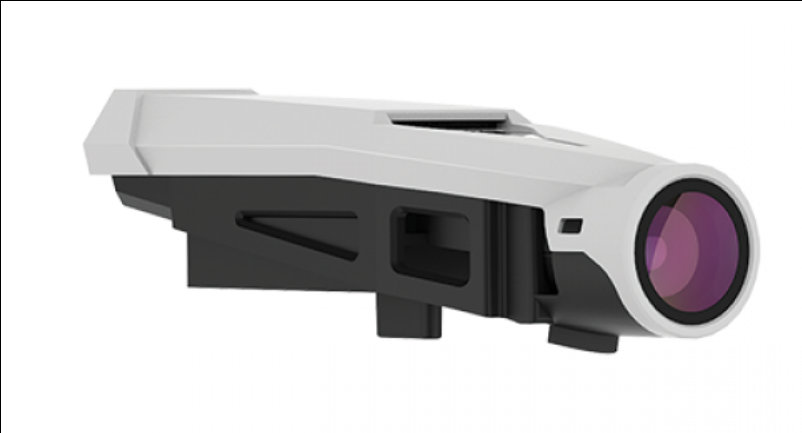
\includegraphics[width=.9\linewidth]{./images/screenshot-02.png}
\end{center}

\begin{center}
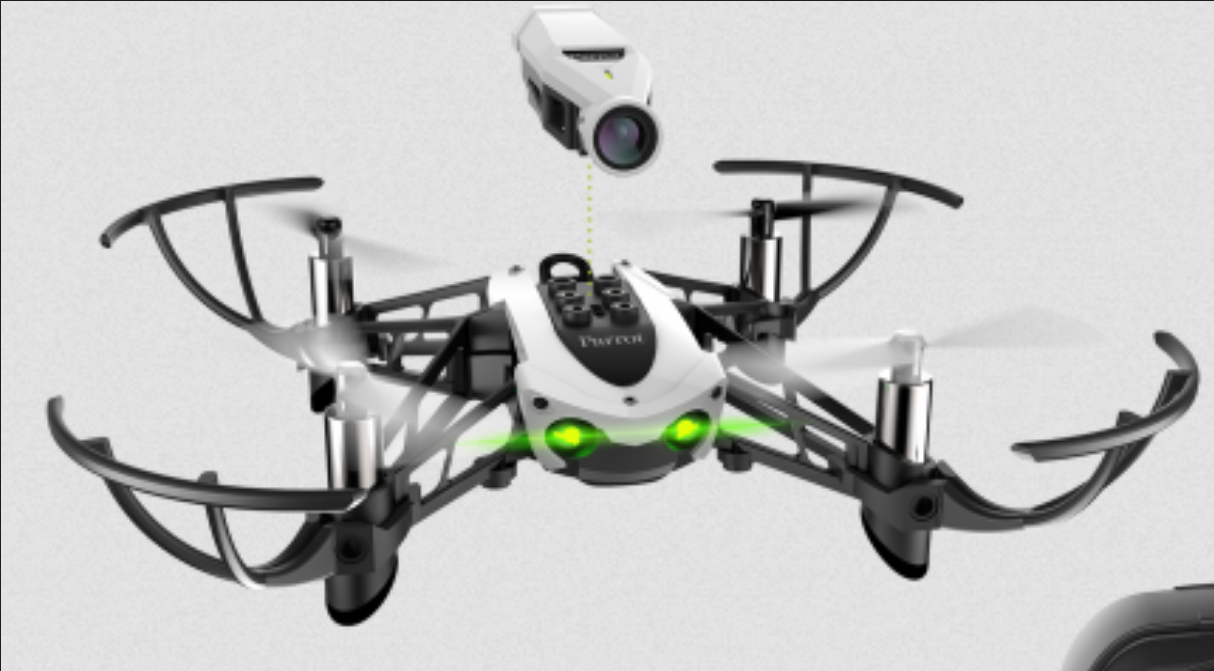
\includegraphics[width=.9\linewidth]{./images/screenshot-03.png}
\end{center}

\subsection{Physical Characteristics}
\label{sec:orgb6f7784}
Need to get a MoI matrix from this
\subsubsection{Weight}
\label{sec:orgfccc059}
Weight: 2.22 oz / 63g (without bumpers or accessories)
Weight with Camera: 73g
\subsubsection{Dimensions}
\label{sec:org32c8f5f}
7.1 x 7.1 in. / 18 x 18 cm with Bumpers
\subsubsection{Rotor Characteristics}
\label{sec:orgbbc489e}

\begin{center}
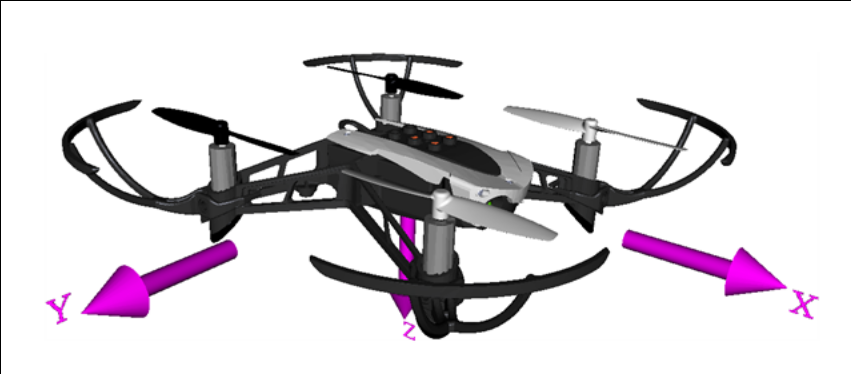
\includegraphics[width=.9\linewidth]{./images/screenshot-04.png}
\end{center}

Right-hand Coordinate Frame centered at Center of gravity.

Rotor \#1 rotates positively with respect to the z-axis. It is located parallel to the xy-plane, -45 degrees from the x-axis.

Rotor \#2 rotates negatively with respect to the body's z-axis. It is located parallel to the xy-plane, -135 degrees from the x-axis.

Rotor \#3 has the same rotation direction as rotor \#1. It is located parallel to the xy-plane, 135 degrees from the x-axis.

Rotor \#4 has the same rotation direction as rotor \#2. It is located parallel to the xy-plane, 45 degrees from the x-axis.
\end{document}
